\documentclass[letterpaper, 12pt]{article}

 
\usepackage[utf8]{inputenc}
\usepackage[T1]{fontenc} 
\usepackage[french]{babel}
\usepackage{amsmath}
\usepackage{textcomp}
\usepackage{tocloft}

\usepackage[letterpaper, left=2.5cm, right=2.5cm, top=2.5cm, bottom=2.5cm]{geometry}
\usepackage{graphicx}
\usepackage{float} 
\usepackage{setspace} 
\usepackage{fancyhdr}      
\usepackage{cite}

\usepackage[pdftex, colorlinks=true, linkcolor=black, citecolor=blue]{hyperref}

\title{Proposé de recherche}
\author{Thomas Dändliker}
\date{\today}

\pagestyle{fancy}
\fancyhead[L]{Proposé de recherche}
\fancyhead[R]{MET-7900}

%%%%%%%%%%%% Fin du préambule %%%%%%%%%%%

\begin{document}

\begin{titlepage}
	\newcommand{\HRule}{\rule{\linewidth}{0.2mm}}     
	
	\begin{figure}[t]
		\begin{minipage}{0.5\textwidth}\large
			\begin{flushleft}
				
\includegraphics[width=5cm]{ULAVAL}
			\end{flushleft}
		\end{minipage}
		\begin{minipage}{0.5\textwidth}\large
			\begin{flushright}
				
\includegraphics[width=6cm]{CRMR}
				
			\end{flushright}
		\end{minipage}
	\end{figure}
	\textsc{ \\[1cm]}
	
	% Titre
	\begin{center}
		\HRule 
		\\[0.5cm]
		{\Large    \textbf{Optimisation de la densité de reboisement en fonction des grades de qualité des bois sciés}}
		\HRule
		\\[0.5cm]
		{\large Proposé de recherche \\
		}
		
	\end{center}
	
	\vfill 
	\begin{center}
		
		\textsc{\large      
			Université Laval\\
			Faculté de foresterie, de géographie et de géomatique\\[3cm]}
	\end{center}

	
	\begin{minipage}{0.5\textwidth}
		\begin{flushleft} \large
			\emph{Auteur:}\\
			Thomas Dandliker 
		\end{flushleft}
	\end{minipage}
	~
	\begin{minipage}{0.5\textwidth}
		\begin{flushright}\large
			\emph{Superviseurs:} \\
			Alexis Achim \\
			Charles Ward \\
		\end{flushright}
	\end{minipage}
	
\end{titlepage}


\renewcommand{\contentsname}{\hfill\bfseries\LARGE Table des matières\hfill} 
\renewcommand{\listfigurename}{\hfill\bfseries\LARGE Table des figures\hfill} 

%%%%%%%%% Table des matières %%%%%%%%%%%

\newpage
\doublespacing
\setcounter{tocdepth}{3}
\tableofcontents
\addtocontents{toc}{\vspace{2cm}}

%%%%%%%%% Table des figures %%%%%%%%%%

\newpage
\doublespacing
\listoffigures

\newpage
\section{Introduction}
\begin{onehalfspace}

Les forêts issues de plantation comptent pour 4\% des forêts mondiales, mais fournissent, à elles seules, 50\% de la production de bois \cite{Miller2009}. Pour la période de 2001 à 2012, avec environ 120 millions de plants plantés annuellement, les résineux représentent presque la totalité des plantations au Québec, soit 98\% \cite{Richard2015}. Depuis 2001, 94\% des plantations sont réalisées avec trois essences: l'épinette noire (56\%), le pin gris (21\%) et l'épinette blanche (17\%) comme l'illustre la figure 1. 

\vspace{12pt}

\begin{figure}[h]
	\centering
	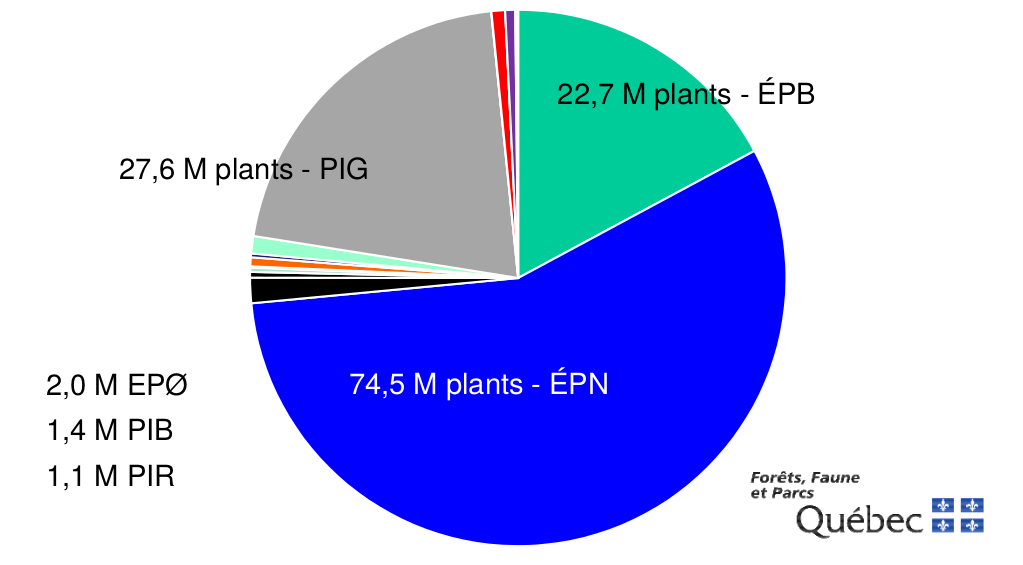
\includegraphics[width=12cm]{Essencesplantees}
	\caption{Essences plantées entre 2001 et 2012 au Québec}
\end{figure}


Ces trois essences font partie du groupe dits SEPM (Sapin, Épinettes, Pins, Mélèzes), qui constitue la  majeure  partie  des  volumes  de  bois  récoltés et transformés au Québec. Ce groupe est à la base de l’approvisionnement des usines produisant du sciage\cite{Gouv2017}. Dans un marché globalisé, cela implique d'optimiser les procédés qui englobent toutes la chaîne de valeur du bois, y compris les scénarios sylvicoles \cite{Gaudreault2010}. 

\vspace{12pt}

Dans ce cadre de rationnalisation, la densité de plantation est un outil ayant une influence importante en sylviculture, puisqu'elle détermine la croissance et les caractéristiques du peuplement \cite{Thiffault2003}. De manière générale, la hauteur dominante, quant à elle, n'est pas influencée par l'espacement entre les tiges \cite{Gizachew2012}. En revanche, lorsque le nombre de tiges par hectare augmente, on a pu observer des augmentations du volume total et de la surface terrière, et, dans le même temps, une diminution du diamètre quadratique moyen. De plus, la mortalité y est aussi plus forte, due à une compétition intraspécifique plus élevée \cite{Groot2016, Will2010}. À l'inverse, à plus faible densité de plantation, on constate un taux de survie plus élevé, ainsi qu'une plus forte croissance en diamètre et en volume par tige \cite{Akers2013}. On y observe également une augmentation du défilement. Ce dernier aspect a une incidence directe sur le volume marchand des tiges. En effet, pour un même diamètre donné, un défilement plus élevé diminue le volume marchand à l'échelle de l'arbre\cite{Pregent1998}. %il te faut aussi présenter le contre argument: en un meme temps, si on a une croissance radiale plus rapide, on sera en mesure de transformer une plus forte proportion du volume en planche. Tu peux citer l'article de StatSAW pour appuyer ça.
Ainsi, deux facteurs entrent en compte lors de la première transformation d'un arbre: le diamètre et la hauteur totale. Ces deux caractéristiques influent sur la composition du panier de produits sciés \cite{Auty2014}, comme par exemple la proportion de sciage. 

\vspace{12pt}

Aussi, l'accroissement plus élevé que l'on constate en plantation modifie les caractéristiques du bois et, de ce fait, a un effet déterminant quant à la valeur et à l'utilisation finale du produit \cite{Zhang2002}. Dans le marché nord-américain, La manière la plus commune d'attribuer une valeur pour les résineux consiste à effectuer un classement visuel des bois sciés comme le fait la norme "National Lumber Grades Authority (NLGA)". Les nœuds (branches), notamment leurs tailles et leurs nombres, sont des caractéristiques importantes à prendre en considération lors du classement des bois sciés \cite{Lemieux2000}. 

\vspace{12pt}

Dans la littérature, un certain nombre d'études soulignent le fait que le DHP de l'arbre a davantage d'effet sur les caractéristiques des branches, que l'espacement initial. Ainsi, les attributs des nœuds peuvent être prédits pour le pin gris et l’épinette noire à partir de données externes de branches, notamment le diamètre des branches \cite{Duchateau2013}. De plus, pour un site donné, les propriétés des noeuds d'épinette noire (\textit{Picea mariana} (Mill.)) sont relativement peu sensibles à l'espacement des arbres, car elles sont largement expliquées par la taille du fût et celle du houppier \cite{Benjamin2009, Zhang2005}. Cela est également observé sur l'épinette de Norvège en Scandinavie \cite{Johansson1992, Makinen1999, Pfister2007}. Enfin, le diamètre de la plus grande branche est positivement corrélé au DHP de l'arbre, quel que soit l'espacement entre les arbres \cite{Hebert2016, Tong2005}. 

\vspace{12pt}

%Il me semble que cette idée cadre plus avec ce que tu disais plus haut sur le défilement. En remontant le paragrpahe, tu éviterais d'y aller dans une séquence: croissance en diamètre - noeuds - croissance en diamètre.
Il est également reconnu que le DHP d'un arbre est, à son tour, étroitement lié à la densité de plantation \cite{Pregent1998}. Plusieurs études vont dans ce sens. Pour le pin gris (\textit{Pinus banksiana} Lamb.), l'espacement des plantations a un effet significatif sur le plus grand diamètre de la branche pour les pins gris dominants \cite{Hebert2016}. Enfin, pour l'épinette blanche (\textit{Picea glauca}), un espacement plus large entre les arbres a tendance à augmenter la largeur des nœuds \cite{Tong2013}. %évite d'utiliser un article, une idée, une phrase. Ici, tes deux idées disent la même chose pour deux espèce différentes. Rassemble ça en une seule idée et place les deux référence à la fin.
Aux vues de ces connaissances, le sylviculteur a une réelle emprise sur la qualité du bois dès sa première décision, qui est celle de choisir la densité de plantation. % voici de nouvelles phrases qui rassemblent tes idées et identifient mieux le besoin de recherche
D'une part, un espacement initial élevé aura l'avantage de stimuler la croissance diamétrale des tiges, ce qui favorisera la production de bois de sciage sur de plus courtes révolutions. D'autre part, le défilement plus élevé et la taille plus élevées des nœuds qui découlent de tels espacements initiaux est susceptible de diminuer le rendement en sciage, leur grade de qualité, et donc la valeur des bois produits. Les sylviculteurs québécois n'ont présentement pas d'outils à leur disposition leur permettant d'évaluer où se situe l'optimum d'espacement initial qui maximiserait la valeur des bois produits.

\vspace{12pt}

Les études menées préalablement sur les branches sont, pour l'instant, toutes limitées à un site en particulier avec des conditions de croissance bien définies (indice de qualité de station, précipitation, température, etc.). En outre, les études évaluant la proportion de sciage proviennent de jeunes peuplements résineux qui ne sont souvent pas encore arrivés à maturité; donc n’ayant pas suivi un scénario sylvicole complet, avec ou sans éclaircies. Pour pallier au manque d'un portrait plus général, la présente étude s’appuie sur un réseau de placettes permanentes établies dans des plantations s'approchant de la maturité à l’échelle de la province de Québec %on dit la province "de" Québec
, ce qui permettra de couvrir de nombreux types de stations ayant des conditions de croissance différentes. 

\vspace{12pt}

%De facon générale, l'association de la taille des nœuds et du défilement peut influer sur la qualité du bois. Toutefois, cette conclusion est appuyée sur des données fragmentaires, notamment sur des arbres d'une trentaine d'années dans les plantations boréales.

% Je t'ai enlevé les deux phrases suivantes qui n'apportaient rien qui n'était pas déjà bien décrit. De manière générale, je trouve que ton introduction fait mal ressortir les avantages possibles d'un espacement plus large. J'en ai ajouté un bout, mais il te faudra développer le réflexe de bien présenter les deux tendances contraires, et donc la recherche d'un optimum, lorsque tu présentes ton projet.
Le présent projet vise à établir un lien entre la future qualité du bois scié et la croissance des arbres à différents espacements pour trois espèces commerciales du Canada, soit l'épinette noire, l'épinette blanche et le pin gris. L'objectif de l'étude est d'évaluer l'effet de différents espacements sur les propriétés du bois d'arbres arrivés à maturité. Plus particulièrement, nous avons cherché à déterminer si une réponse positive du DHP à un espacement plus grand affecterait le classement du bois et la proportion de sciage.

\vspace{12pt}

%raffinement de l'hypothèse
Nous avons émis l'hypothèse qu'une densité de reboisement plus faible que celui appliqué présentement au Québec, soit 2 m, augmenterait le diamètre à l'échelle de l'arbre, ce qui augmenterait le rendement en sciage sans diminuer outre mesure le classement des sciages. Cette hypothèse implique donc que l'optimum de rendement en valeur des produits se situerait à un espacement initial inférieur à celui utilisé en ce moment. 

\section{Matériel et méthodes} % matériel toujours singulier en français dans ce contexte

\subsection{Aire d'étude}

L'expérience sera réalisée à l'échelle de la province de Québec et elle mettra à profit le réseau des placettes permanentes de la Direction de la Recherche Forestière (DRF). Les essences étudiées sont l'épinette noire (\textit{Picea mariana} (Mill.)), l'épinette blanche (\textit{Picea glauca}) et le pin gris (\textit{Pinus banksiana} Lamb.).Des mesures préliminaires ont été prises à l'été et automne 2018 et elles seront complétées au printemps et à l'été 2019 dans une centaine de plantations monospécifiques âgées de 30 ans environ. Les plantations sélectionnées n'ont subi aucune éclaircie précommerciale. %il te faudrait décrire la méthode de sélection de tes plantations. Le principe de sélection et la stratification sont deux éléments importants du proposé. 

Les placettes permanentes utilisées sont des unités d'échantillonnage circulaires d'une superficie de 400 m$^{2}$ \cite{MFFP2016}. Dans le cadre de ce projet, les données suivantes ont été relevées sur un nombre déterminé % il est fondamentalement important que tu spécifies le nombre d'arbres
 d'arbres: essence de l'arbre, le diamètre à hauteur de poitrine (DHP) et les caractéristiques de la plus grosse branche sur les cinq premiers mètres de la tige. 

\subsection{Mesures de branches} % Cette sectio nrequiert du travail parce que la méthode de sélection n'est pas claire

La classification des branches se fait d’abord sur les arbres études compris dans les étages dominants et codominants (8 à 10 arbres par placette %comment sot-ils choisis?
) et, en second, sur les arbres listés dans le formulaire électronique de DendroDIF. %clarifier cette dernière information
En prévision du fait que certains défaut auront apparu sur les arbres après le dernier mesurage effectué dans les placette, une liste sera construite de tous les arbres respectant les quatre critères de sélection. %tu ne devrais pas parler des critères de sélection sans les avoir présentés préalablement, ou immédiatement après.
Cette liste servira à compléter la sélection des arbres jusqu’à une concurrence de 20 arbres et elle n’est pas triée en ordre prioritaire de sélection. Les arbres sont sélectionnés prioritairement sur la ligne à proximité du centre de la placette (ligne en rouge et pleine sur la Figure~\ref{select}) %le principe d'utilisation de latex est de tout automatiser pour éviter les erreurs comme celle-ci (il s'agit de la figure 2). Voici comment régler le problème. Corriger partout dans le texte
, suivi sur la ligne le plus vers le nord magnétique, suivi sur les lignes adjacentes jusqu’à atteindre la ligne centrale de la placette  (lignes en bleu sur  la Figure 1) et, si nécessaire, sur les autres lignes adjacentes à la ligne du centre et en priorisant toujours celles orientées vers le nord magnétique (lignes en jaune sur la Figure 1).

\vspace{12pt}

\begin{figure}
	\centering
	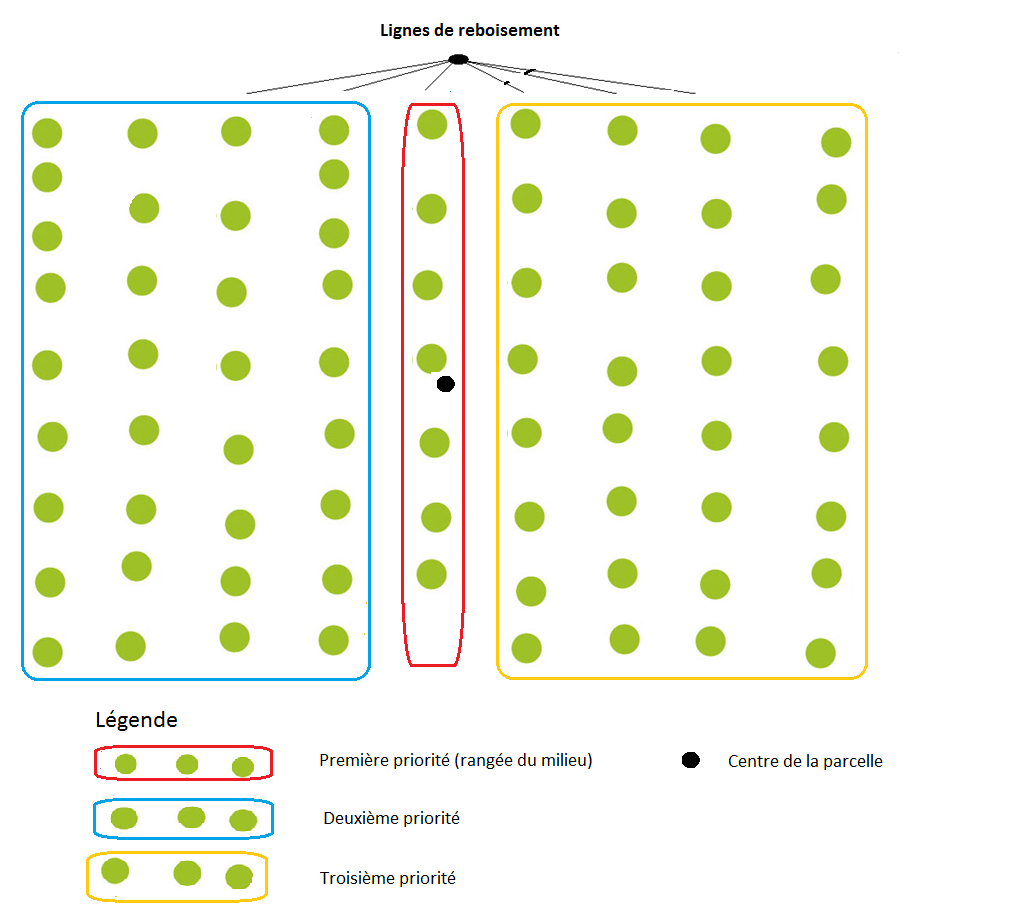
\includegraphics[width=10cm]{Figure1}
	\caption{Priorité de sélection des arbres pour la classification des branches}
	\label{select}
\end{figure}

Pour chaque arbre sélectionné, la circonférence de la bille de pied de 4,9 m (16 pieds) sera ensuite divisée en quatre faces égales (Figure 2). Les faces A et C seront alignées sur la ligne de plantation et les faces B et D seront donc perpendiculaires à la ligne de plantation. La face A sera celle orientée le plus vers le nord magnétique et elle est identifiée par un trait de peinture vertical de 10 cm, à la base du tronc, à l’aide de peinture.

\vspace{12pt}

\begin{figure}[H]
	\centering
	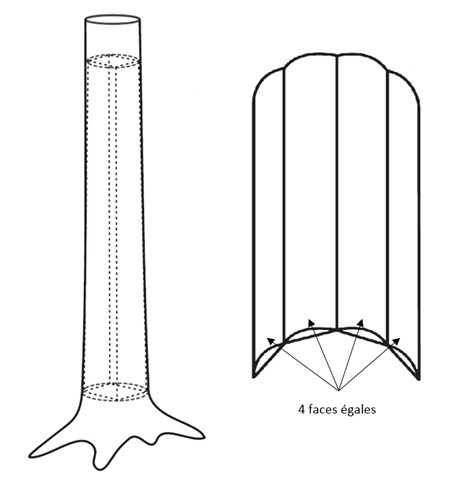
\includegraphics[width=6cm]{Figure2}
	\caption{Division de la circonférence de la bille de pied en quatre faces égales}
\end{figure}

\vspace{12pt}

Le diamètre de la plus grande branche sera ensuite mesuré sur chacune des faces, selon les six classes suivantes %ici il te faut expliquer la logique derrière ces classes de grosseurs. Ton rôle dans un proposé est de montrer que ton projet se tient. Tu dois donc "vendre" tes méthodes pour montrer qu'elles sont réfléchies. C'est cet aspect qui manque présentement dans cette section.
 :

\begin{figure}[H]
	\centering
	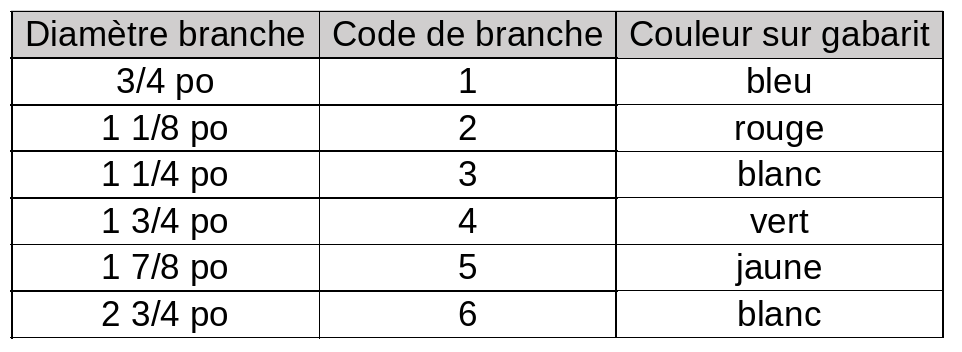
\includegraphics[width=10cm]{Code}
\end{figure}

\vspace{12pt}

La plus grosse branche sera sélectionnée jusqu’à une hauteur de 5,23 m (17 pieds), à partir du sol, et par la suite mesurée à l’aide du gabarit métallique. À cet effet, des perches télescopiques et des gabarits métalliques, identifiant les six classes de diamètres de branches, ont été fournies aux personnes qui réaliseront les mesures.

\vspace{12pt}

La mesure des branches se décline comme suit:

\begin{enumerate}
	
\item Déployer la perche téléscopique pour atteindre une longueur de 3,93 m. Cette longueur correspond à la longueur totale de la perche sans le gabarit. Ainsi elle débute au niveau du trait rouge présent sur le gabarit métallique (Figure 4) jusqu'à l'autre extrémité de la perche téléscopique.

\item Se placer devant la face à mesurer avec la perche téléscopique munie du gabarit métallique.

\item Positionner la base de la perche à  1,3 m du sol : prendre la perche téléscopique par la base, et la soulever jusqu'au niveau du DHP, identifié par un trait de peinture sur l'arbre (Figure 5). Cette position permet de délimiter la hauteur totale de 5,23 m, hauteur qui sert à étudier les branches.

\item Chercher la branche la plus grosse sur la face étudiée et la mesurer à l’aide du gabarit métallique (Figure 4). Inscrire dans le formulaire Dendrodif le «code diamètre branche» selon le tableau ci-dessus (Tableau 1), correspondant à la plus grosse branche. Pour chacune des branches, identifier et inscrire dans le formulaire Dendrodif, son «état branche» : vivante = \textbf{V}, ou morte = \textbf{M}.  De plus, inscrire dans le formulaire Dendrodif, son «angle insertion branche» : 45° et moins = \textbf{- 45}, ou 45° et plus = \textbf{+ 45}.

\end{enumerate}

\vspace{12pt}
 
Voir exemple ci-dessous de prise de mesures dans le formulaire Dendrodif :

\begin{figure}[H]
	\centering
	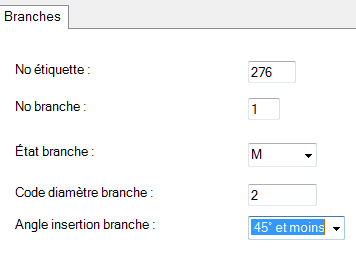
\includegraphics[width=5cm]{Figure3}
	\caption{Interface DendroDif}
\end{figure}

\begin{figure}[H]
	\centering
	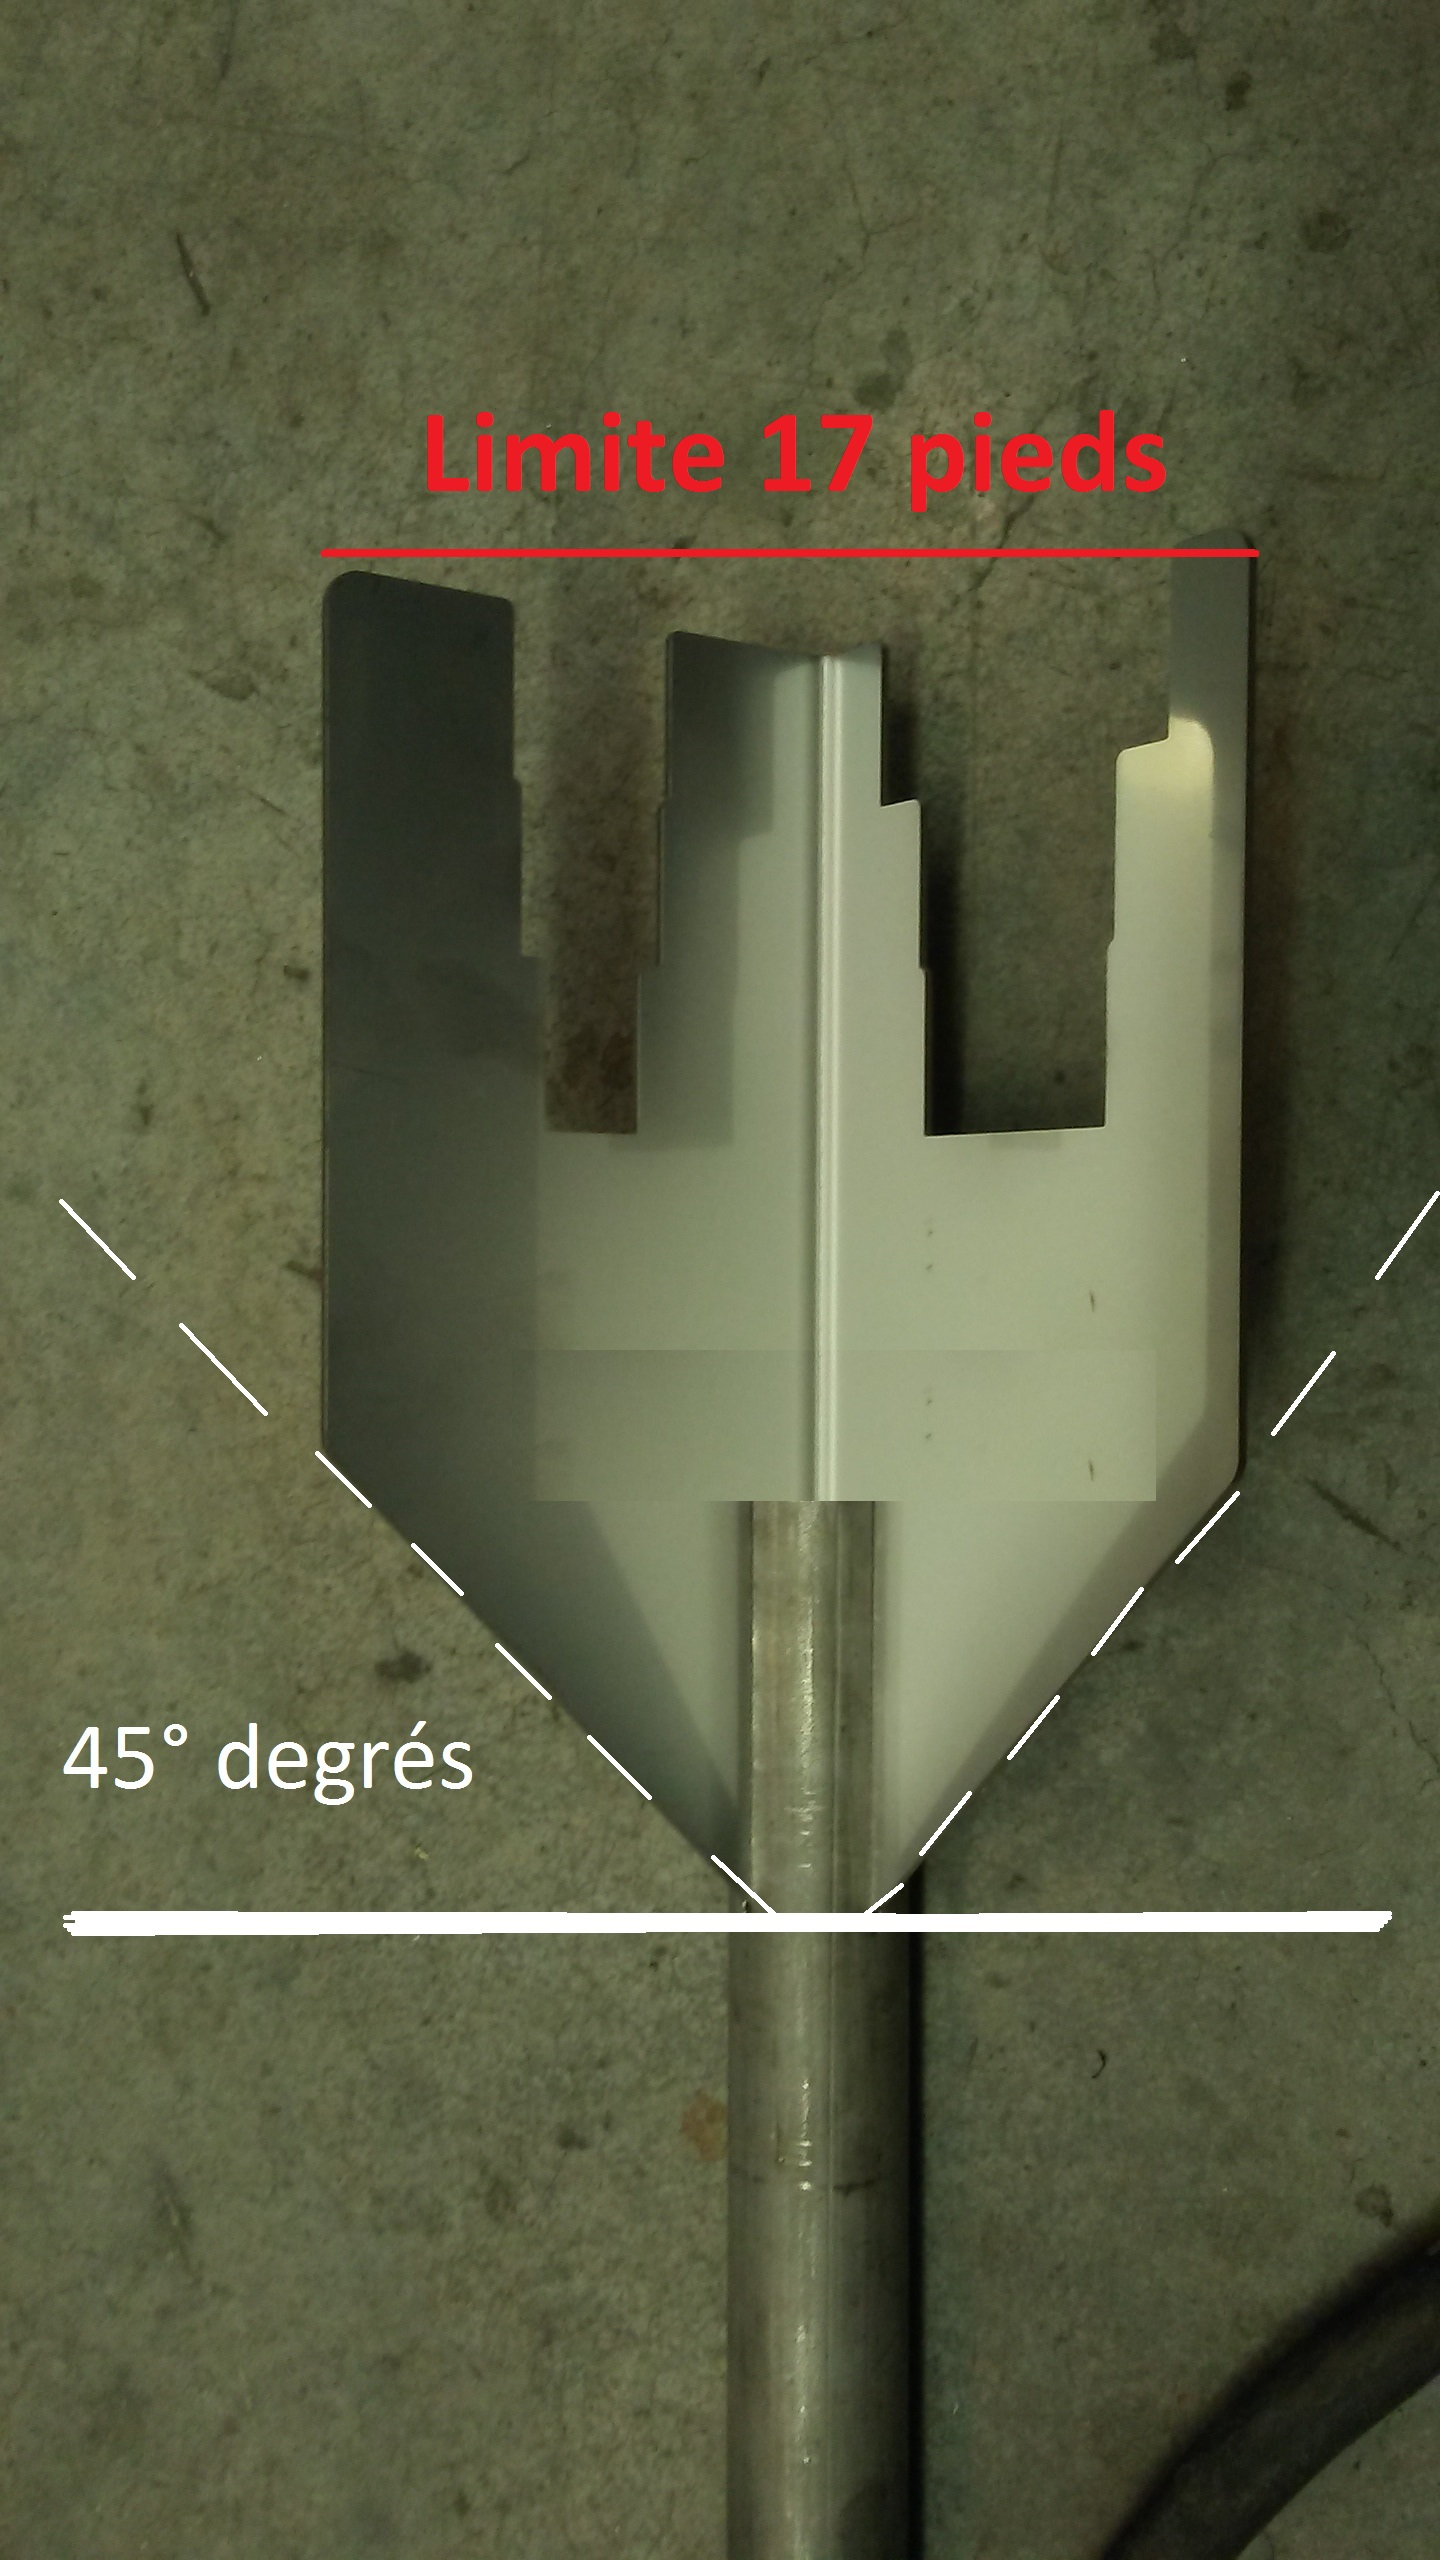
\includegraphics[width=5cm]{Figure4}
	\caption{Gabarit métallique}
\end{figure}

\begin{figure}[H]
	\centering
	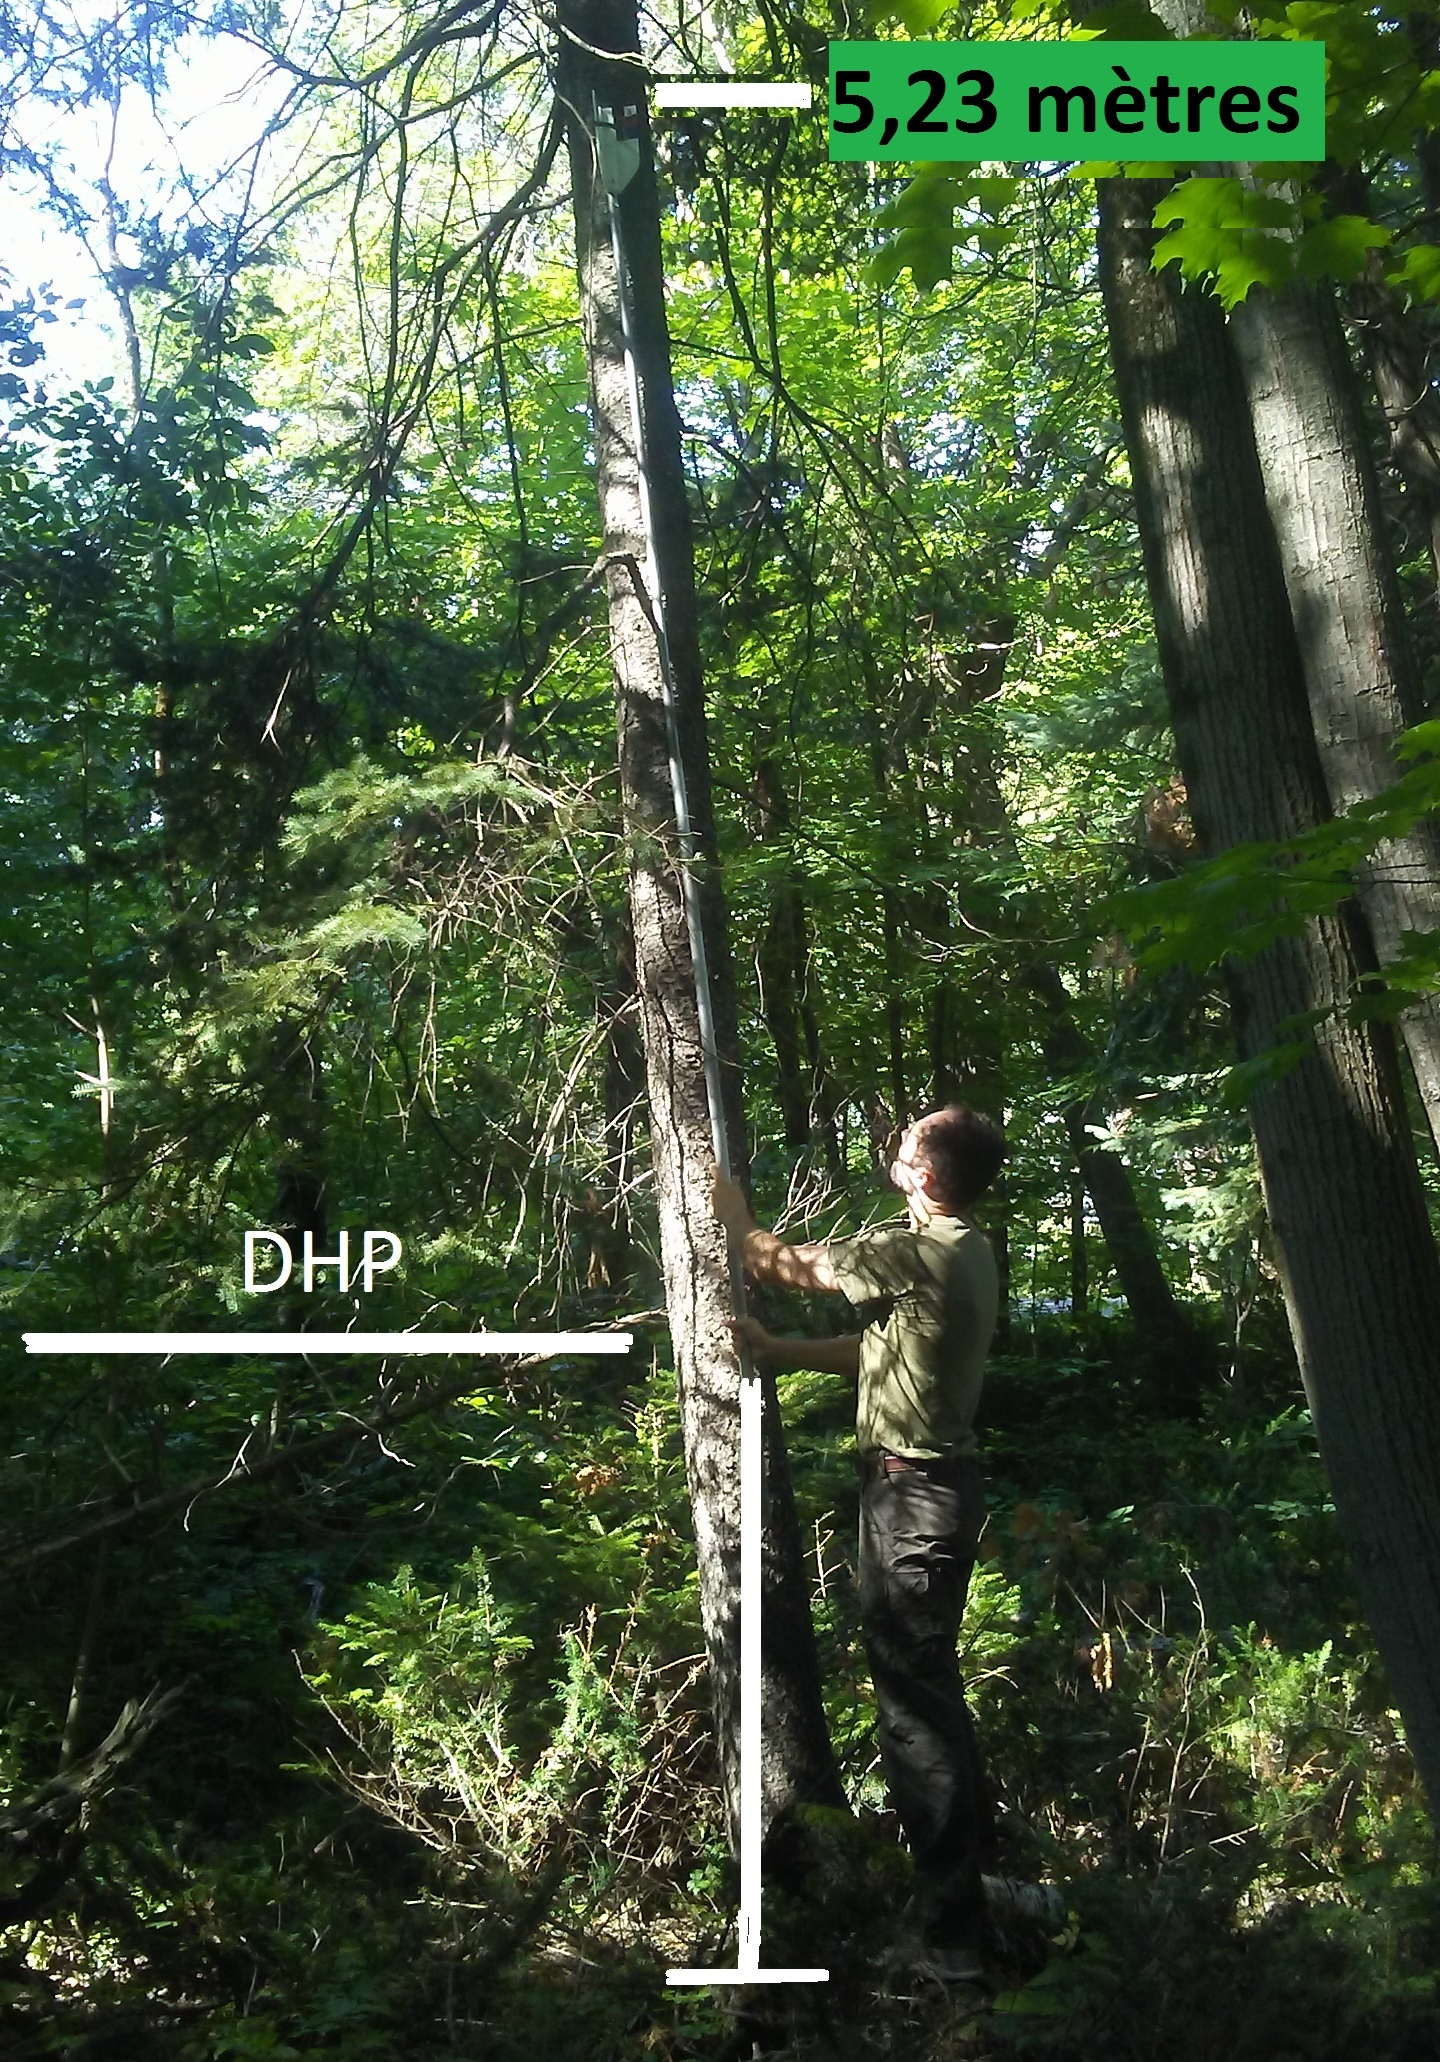
\includegraphics[width=5cm]{Figure5}
	\caption{Détermination de la hauteur de 5,23 m}
\end{figure}

\subsubsection{Analyse statistique}

Plusieurs données seront récoltées sur les arbres dans toutes les placettes permanentes. Pour l'analyse de ces données, les variables dépendantes seront les suivantes: le numéro d'encoche (grosseur de la branche), l'inclinaison de la branche, et l'état de la branche. Quant aux variables explicatives, il y aura : l'essence, la densité de plantation (plant/ha), l'IQS et l'exposition. Concernant les paramètres environnementaux, nous utiliserons principalement l'exposition, car elle peut favoriser la croissance du houppier sur la face la plus ensoleillée. Par une technique de régression multinomiale, il sera possible d'estimer la proportion des faces se ayant une taille de nœuds donnée pour différents scénarios d'espacements. Il sera ensuite possible d'estimer dans quelle mesure un espacement initial plus large est susceptible d'engendrer des déclassements de la qualité des planches. 

\subsection{Modélisation du défilement et de la composition du panier de produits}

À l’aide d’un simulateur d’éclaircies créé par la Direction de la Recherche Forestière (Guy Prégent) %peux-tu citer le simulateur plutôt que son auteur?
, il sera possible de déterminer le DHP quadratique moyen et la hauteur dominante des tiges à maturité en fonction: de l’essence, de l’IQS, de la densité de reboisement et du scénario sylvicole (0, 1 ou 2 éclaircies). 

%Les idées incluses dans ce prochain paragraphe appartiennent plus à l'intro. Ici, on veut savoir comment tu fais
Dans un contexte de marché de plus en plus compétitif, et où les coûts d'extraction pour la ressource et la fabrication des produits du bois augmentent, il devient primordial de maximiser la création de valeur lors de la première transformation \cite{Briggs2010, Walker2013}. Depuis plusieurs décénnies, des simulateurs informatiques de sciages sont utilisés dans le secteur des transformations primaire et secondaire comme stratégie pour optimiser la valeur des produits \cite{FPInnovations2014}. Plusieurs études ont intégré avec succès les variabilités de la taille des arbres (tels que le diamètre de la tige, la hauteur totale de l’arbre ou la conicité de la tige) dans des modèles permettant de prédire le volume ou la valeur lors de la transformation \cite{Barrette2012,Liu2007}.


Afin de simuler la transformation primaire, FPInnovations a développé Optitek, un logiciel qui utilise les données acquises à partir de scanners laser pour donner une représentation tridimensionnelle de la forme réelle de la tige \cite{FPInnovations2014}. Toutefois, ce logiciel demande une compréhension fine de la transformation primaire du bois pour être bien utilisé. Ce niveau de compréhension dépassant le cadre de cette étude, nous utiliserons plutôt une simplification du modèle qui tient compte du DHP et de la hauteur des arbres pour prédire la composition du panier de produits déterminée par Optitek. Ce méta-modèle statistique nommé STATSAW \cite{Auty2014} est paramétré pour l'épinette noire. À défaut d'avoir d'autres modèles, nous utiliserons STATSAW aussi pour l'épinette blanche et le pin gris.

\section{Résultats escomptés}
% à reformuler en fonction de la nouvelle hypothèse. Je pense que tu devrais dire que l'espacement initial plus large pourrait donner de meilleurs résultats, mais que ça peut dépendre des espèces. Comme le pin gris fait de plus gros noeuds, il est possible que l'optimum se situe à une valeur plus faible d'espacement.
On s’attend à une relation entre la densité de plantation et les propriétés du bois (proportion de sciage, grosseur des branches). Le défilement est bien documenté sur les trois essences, ce qui permettra de bien alimenter le simulateur Optitek en données pour prévoir une valeur par arbre. Les ajustements avec le modèle STATSAW étant initialement paramétrés pour l'épinette noire, il y aura nécessairement une incertitude pour l'épinette blanche et le pin gris quant à la projection du panier de produits. Toutefois, on suppose une augmentation de la proportion de sciage pour toutes les essences au fur et à mesure que la densité diminue. 

\vspace{12pt}
Pour le diamètre de la plus grosse branche, on s'attend à observer une augmentation de la grosseur des branches à de plus fortes densités. En effet, la hausse de la mortalité interspécifique devrait libérer de l'espace aux arbres résiduels et favoriser leurs développement de houppier et donc des branches. 





\section{Conclusion}

À la lumière des résultats obtenus, des recommandations pourront être formulées auprès des praticiens en régions pour les sensibiliser aux effets de la densité de reboisement sur les caractéristiques du bois. En  termes  économiques,  si  les caractéristiques du bois ne se dégradent pas trop rapidement au fur et à mesure qu'on diminue la densité de plantation,  il peut être envisageable d'abaisser le nombre de tiges à l'hectare et donc de réduire les  coûts  de  plantation. Une autre retombée espérée est de pouvoir créer, à long terme, des bois issus de plantations ayant le meilleur panier de produits possible. 

\end{onehalfspace}

\section{Échéancier}

\begin{figure}[H]
	\centering
	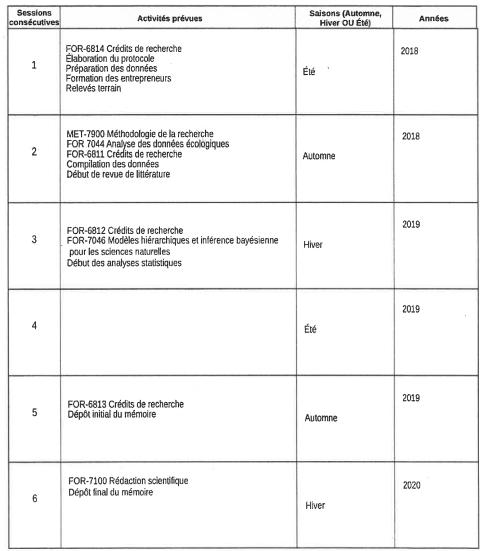
\includegraphics[width=15cm]{Calendrier}
	\caption{Calendrier des activités}
\end{figure}


\newpage

\nocite{*}
\bibliographystyle{unsrt}
\bibliography{biblio}

\end{document}